\documentclass[
  bibliography=totoc,     % Literatur im Inhaltsverzeichnis
  captions=tableheading,  % Tabellenüberschriften
  titlepage=firstiscover, % Titelseite ist Deckblatt
]{scrartcl}

% Paket float verbessern
\usepackage{scrhack}

% Warnung, falls nochmal kompiliert werden muss
\usepackage[aux]{rerunfilecheck}

% unverzichtbare Mathe-Befehle
\usepackage{amsmath}
% viele Mathe-Symbole
\usepackage{amssymb}
% Erweiterungen für amsmath
\usepackage{mathtools}

% Fonteinstellungen
\usepackage{fontspec}
% Latin Modern Fonts werden automatisch geladen
% Alternativ zum Beispiel:
%\setromanfont{Libertinus Serif}
%\setsansfont{Libertinus Sans}
%\setmonofont{Libertinus Mono}

% Wenn man andere Schriftarten gesetzt hat,
% sollte man das Seiten-Layout neu berechnen lassen
\recalctypearea{}

% deutsche Spracheinstellungen
\usepackage[ngerman]{babel}


\usepackage[
  math-style=ISO,    % ┐
  bold-style=ISO,    % │
  sans-style=italic, % │ ISO-Standard folgen
  nabla=upright,     % │
  partial=upright,   % │
  mathrm=sym,        % ┘
  warnings-off={           % ┐
    mathtools-colon,       % │ unnötige Warnungen ausschalten
    mathtools-overbracket, % │
  },                       % ┘
]{unicode-math}

% traditionelle Fonts für Mathematik
\setmathfont{Latin Modern Math}
% Alternativ zum Beispiel:
%\setmathfont{Libertinus Math}

\setmathfont{XITS Math}[range={scr, bfscr}]
\setmathfont{XITS Math}[range={cal, bfcal}, StylisticSet=1]

% Zahlen und Einheiten
\usepackage[
  locale=DE,                   % deutsche Einstellungen
  separate-uncertainty=true,   % immer Unsicherheit mit \pm
  per-mode=symbol-or-fraction, % / in inline math, fraction in display math
]{siunitx}

% chemische Formeln
\usepackage[
  version=4,
  math-greek=default, % ┐ mit unicode-math zusammenarbeiten
  text-greek=default, % ┘
]{mhchem}

% richtige Anführungszeichen
\usepackage[autostyle]{csquotes}

% schöne Brüche im Text
\usepackage{xfrac}

% Standardplatzierung für Floats einstellen
\usepackage{float}
\floatplacement{figure}{htbp}
\floatplacement{table}{htbp}

% Floats innerhalb einer Section halten
\usepackage[
  section, % Floats innerhalb der Section halten
  below,   % unterhalb der Section aber auf der selben Seite ist ok
]{placeins}

% Seite drehen für breite Tabellen: landscape Umgebung
\usepackage{pdflscape}

% Captions schöner machen.
\usepackage[
  labelfont=bf,        % Tabelle x: Abbildung y: ist jetzt fett
  font=small,          % Schrift etwas kleiner als Dokument
  width=0.9\textwidth, % maximale Breite einer Caption schmaler
]{caption}
% subfigure, subtable, subref
\usepackage{subcaption}

% Grafiken können eingebunden werden
\usepackage{graphicx}

% schöne Tabellen
\usepackage{tabularray}
\UseTblrLibrary{booktabs, siunitx}

% Verbesserungen am Schriftbild
\usepackage{microtype}

% Literaturverzeichnis
\usepackage[
  backend=biber,
]{biblatex}
% Quellendatenbank
\addbibresource{lit.bib}
\addbibresource{programme.bib}

% Hyperlinks im Dokument
\usepackage[
  german,
  unicode,        % Unicode in PDF-Attributen erlauben
  pdfusetitle,    % Titel, Autoren und Datum als PDF-Attribute
  pdfcreator={},  % ┐ PDF-Attribute säubern
  pdfproducer={}, % ┘
]{hyperref}
% erweiterte Bookmarks im PDF
\usepackage{bookmark}

% Trennung von Wörtern mit Strichen
\usepackage[shortcuts]{extdash}

\author{%
  Vincent Wirsdörfer\\%
  \href{mailto:vincent.wirsdoerfer@udo.edu}{authorA@udo.edu}%
  \and%
  Joris Daus\\%
  \href{mailto:joris.daus@udo.edu}{authorB@udo.edu}%
}
\publishers{TU Dortmund – Fakultät Physik}

\usepackage{wrapfig}

\begin{document}

\section{Zielsetzung}
\label{Zielsetzung}

\noindent Das Ziel des im folgend protokollierten Versuchs besteht in der Bestimmung der Wellenlänge eines Lasers und des 
Brechungsindex von Luft. Wie dem Versuchstitel bereits zu entnehmen ist, soll dies unter Zuhilfenahme eine Michelson 
Interferometers geschehen.

\section{Theorie}
\label{sec:Theorie}

Licht kann aufgrund von Welleneigenschaften als elektromagnetische Welle dargestellt werden. Dabei sind die elektrische 
Feldstärke $\vec{E}$ und die magnetische Feldstärke $\vec{B}$ jeweils orhtogonal zur Propagationsrichtung der Welle. Mit einem 
Wellenvektor $\vec{k}$ in Ausbreitungsrichtung der Welle gilt dementsprechend $\vec{E} \perp \vec{B} \perp \vec{k}$. Dies wird in 
der untenstehenden Abbildung visualisiert.

\begin{figure}
    \centering
    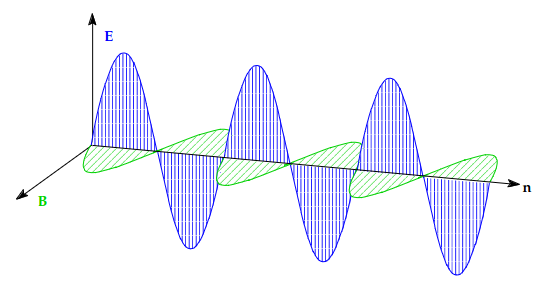
\includegraphics[height=5cm]{EM_Welle.png}
    \caption{Licht als elektromagnetische Welle\cite{Versuchsanleitung_v401}.}
    \label{fig:EMWelle}
\end{figure}

\noindent Die Geschwindigkeit $c$ der Welle berechnet sich durch $c = \lambda\cdot{}f$, wobei $\lambda$ die Wellenlänge und $f$ die Frequenz 
der Welle beschreibt. Großen Anteil an den optischen Eigenschaften der EM-Welle hat die elektrische Feldstärke, beschrieben durch 

\begin{equation*}
%\label{eqn:EFeld}
    \vec{E}\left(\vec{x},t\right) = \vec{E}_0\sin\left(\omega{}t - kx\right),
\end{equation*}

\noindent wobei $\omega = 2\pi{}f$ die Kreisfrequenz und $k = \sfrac{2\pi}{\lambda}$ ist. Die Intensität $I$ ist dabei proportional 
zum Betragsquadrat der elektrischen Feldstärke.\\

\noindent Bei der Überlagerung zweier monochromatischer Wellen treten Interferenzeffekte auf. Abhängig von der Phasenbeziehung $\increment\varphi$
beider Wellen, kann die Gesamtintensität verstärkt oder abgeschwächt werden. Ein Ausdruck für die resultierende Intensität ist 

\begin{equation}
\label{eqn:Intensitaet}
    I = I_1 + I_2 + 2\sqrt{I_1I_2}\cos\left(\varphi_{12}\right)
\end{equation}

\noindent Die Extremfälle konstruktiver bzw. destruktiver Interferenz werden in der folgenden Abbildung veranschaulicht:

\begin{figure}
    \centering
    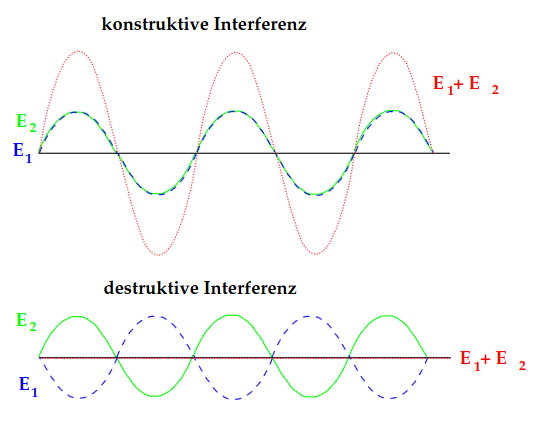
\includegraphics[height=5cm]{Interferenz.png}
    \caption{Interferenz monochromatischer Wellen\cite{Versuchsanleitung_v401}.}
    \label{fig:Interferenz}
\end{figure}

\noindent Natürliche Lichtquellen sind aufgrund spontaner Emission und unkorrelierter Wellenzüge nicht fähig zur Interferenz, weshalb der 
phasenabhängige Term aus \eqref{eqn:Intensitaet} vernachlässigt wird. Im Gegensatz dazu sind monochromatische Wellen mit fester 
Phasenbeziehung interferenzfähig und werden als \emph{kohärent} bezeichnet. Die spektrale Bandbreite $\increment{}f$ und die Länge des 
Wellenzugs $\increment{}l$ sind invers proportional zueinander ($\increment{}f\cdot\increment{}l = c$). Deshalb führt eine geringe 
spektrale Bandbreite zu einer großen Kohärenzlänge und umgekehrt.\\
    Interferometer bieten eine Möglichkeit, Längenänderung oder Brechungsindizes mittels interferierendem Licht zu bestimmen.
    Beim hier verwendeten \emph{Michelson Interferometer} spaltet eine Teilerplatte ein Lichtbündel in zwei zueinander senkrechte 
    Strahlenbündel auf. Mittels Reflexion an zwei Spiegeln können beide Lichtbündel erneut entgegen geschickt werden, sodass diese miteinander 
    interferieren.
%
%\begin{minipage}{0.5\textwidth}
%\end{minipage}
%\hfill
%\begin{minipage}{0.5\textwidth}
%%    \centering
%    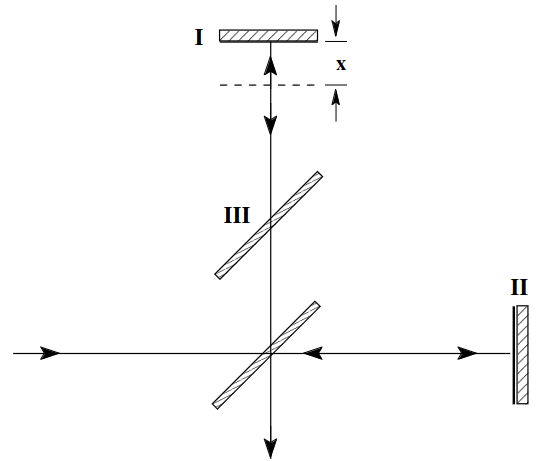
\includegraphics[width=\textwidth]{Michelson_Interferom.png}
%\end{minipage}
%
\begin{wrapfigure}{R}{0.5\textwidth}
    \vspace{-20pt}
    \begin{center}
        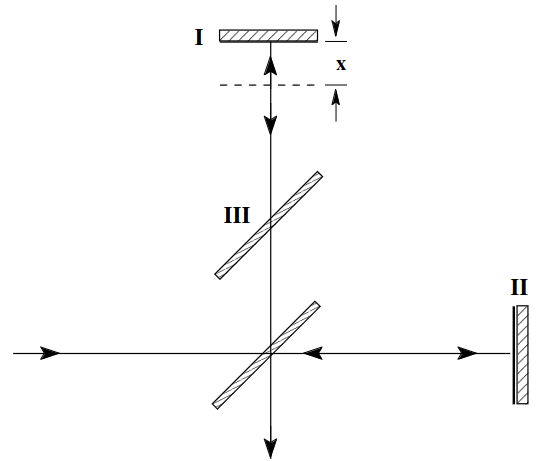
\includegraphics[width=0.5\textwidth]{Michelson_Interferom.png}
    \end{center}
\end{wrapfigure}

\noindent Auf dem Schirm im überlagerten Lichtweg ist ein Interferenzmuster zu erkennen. Zur Kompensation der unterschiedlich langen 
Wegstrecken der Strahlenbündel, wird dem reflektierten Strahlengang eine Glasplatte hinzugefügt. Über das Verschieben einer der 
Spiegel um $\sfrac{\lambda}{2}$ werden die Interferenzmaxima und -Minima auf den Schirm \enquote{vertauscht}. Somit kann auf Grundlage 
der Wechselhäufigkeit $z$ der Minima und Maxima bei bekannter Wellenlänge $\lambda$ die Längenänderung $x$ über 

\begin{equation*}
%\label{eqn:Laenge}
    \lambda = \frac{2x}{z}
\end{equation*}

\noindent berechnet werden.

\section{Vorbereitung}

Die Literaturwerte der Brechungsindizes von Luft, Kohlenstoffmonoxid und Kohlenstoffdioxid lauten wie folgt.

\begin{align}
    n_\text{Luft} &= 1.00029\text{\cite{Brechzahl_Luft}}\\ 
    n_\text{CO} &= 1.0003\text{\cite{Brechzahl_CO}}\\ 
    n_\text{CO$_2$} &= 1.0004\text{\cite{Brechzahl_CODI}}\\
\end{align}

%\section{Fehlerrechnung}
\end{document}